%************************************************
\chapter{Frank Hertz}
%************************************************
\begin{flushright}
February 16, 2013
\end{flushright}
\section{Aim}
	To experimentally verify that atomic energy levels are discrete, using the frank-hertz setup.
\section{Apparatus}
	Frank Hertz Apparatus, An Oscilloscope, a few connecting wires and a camera or tracing paper

\section{Theory}
	\subsection{Rationale Behind the Experiment}
		This experiment is very fascinating, for it experimentally, using a rather naive method, proves the atomic energy levels are discrete.
		\par
		The basic idea is to bombard atoms with progressively higher energy electrons, and measure the current of these electrons. When the electrons have specific, discrete energy values, they collide plastically with the atoms and the current drops. If we plot the energy of the electrons against the current obtained, the difference in energy between two consecutive valleys (in the graph), will give the energy difference between two atomic states.
	\subsection{Experimental Setup}	
		The detailed setup of the experiment is beyond the scope of this report. However, to a first approximation, the setup can be understood in terms of a triode as given in \autoref{e2_circuit}. An electrode is heated by flow of electric current. This thermal energy, acquired by the electrons, if exceeds the binding energy of the electron with the metal, results in ejection of electrons from the metal surface. (Of course there would be a distribution of thermal energy, however, here we are not getting into the quantitative details) There's another electrode, called the grid, which is at a higher potential with respect to the cathode (the first electrode, which releases electrons). This potential is maintained to a desired value by a variable potential source. Most electrons, get through the grid, and gain an energy equivalent to $eV$ where $e$ is the charge of an electron, and $V$ is the potential difference between the electrodes. So far so good. Now we introduce a third electrode. The magnitude of potential difference between the grid and the cathode is greater than that between the grid and the third electrode (call it $V_2$), viz. $|V|>|V_2|$. Consequently, the current that flows through the third electrode, will be constituted by electrons that have an energy greater than $eV_2$. The entire setup is enclosed within a vacuum tube, with Argon atoms.
		\par
		Now we vary $V$ to increase the maximum kinetic energy and measure the current $I$ through the third electrode. The current is expected to increase in a known fashion (precise details are not relevant at the moment) in the absence of Argon. In the presence of Argon, the current drops periodically to a minima, at constant voltage differences.
\section{Observations and Calculations}
	Observations have been appended at the end of this experiment. \\

	\begin{figure}[bth]
		\begin{center}
			
\includegraphics[width=1.0\linewidth]{gfx/e2_circuit}
		\end{center}
	\caption[Simplified schematic of the Setup]{Simplified schematic of the Setup}
	\label{e2_circuit}
	\end{figure}


	\begin{figure}[bth]
		\begin{center}
			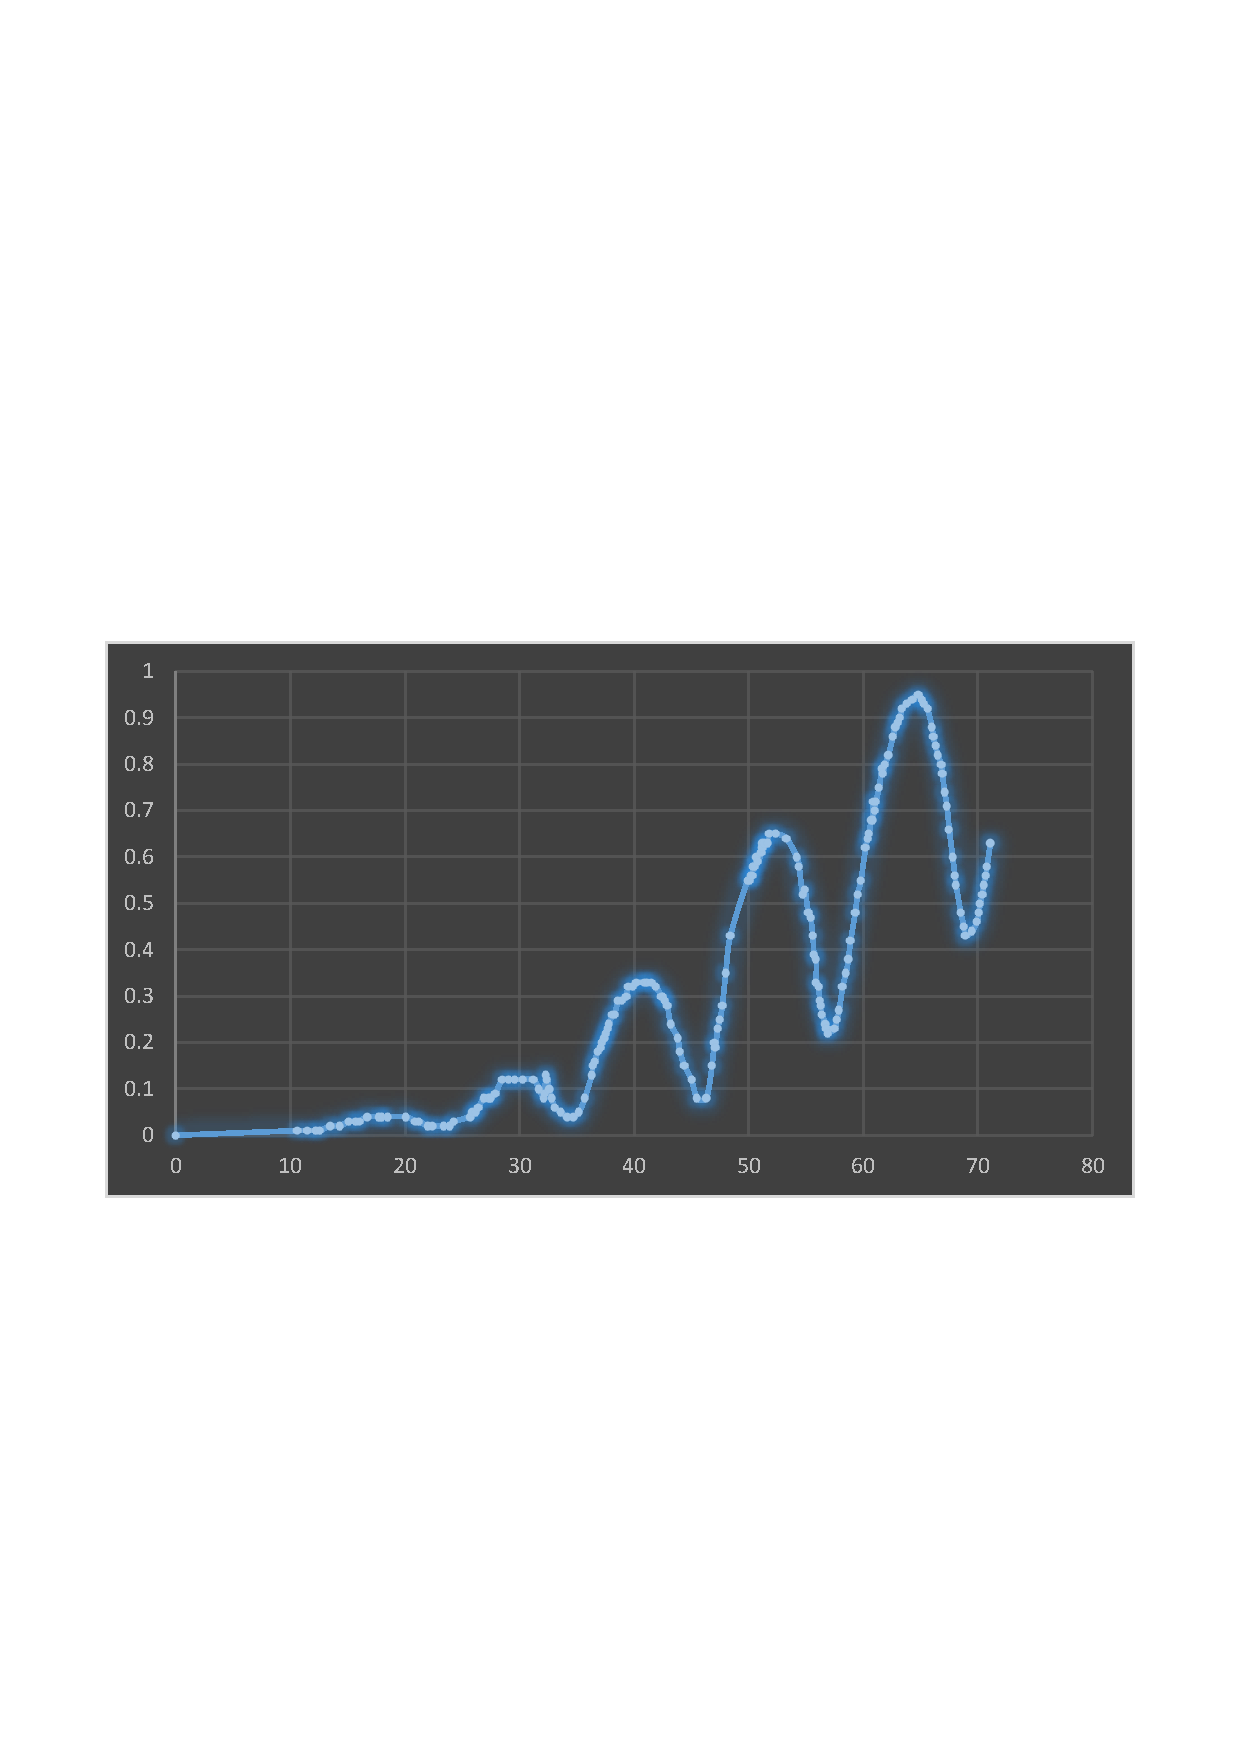
\includegraphics[width=1.3\linewidth]{gfx/e2_result.pdf}
		\end{center}
	\caption[Graph for the Manual Mode]{Graph for the Manual Mode}
	\label{e2_result}
	\end{figure}

\section{Procedure}
	The procedure has been influenced heavily by the one given in the Physics Lab Manual, provided to us, during the course, PHY212, 2013.
	\begin{enumerate}
		\item Before switching on the power, it was made sure that the control knobs are at their minimum and the current multiplier knob is set to $10^{-7}$.
		\begin{enumerate}
		\item Manual
			\item The Manual mode was selected using the Manual-Auto switch.
			\item Turned the display selector to $V_{G_1K}$ and adjusted the corresponding knob to read $1.5V$ on the display
			\item Next, $V_{G_2A}$ was selected and set to $7.5V$
			\item Now, the $V_{G_2K}$ knob was turned and the variation of the current (these correspond to $V$ and $I$ discussed in the theory) noted, with increase in voltage from zero.
			\item The graph for the same is plot and average distance between two successive maxima (or minima) is calculated. This gives the first excitation potential for Argon.
		\item Automatic
			\item Scanning mode was selected by turning the Manual-Auto switch to auto.
			\item The instruments X, Y, G sockets were put in the corresponding sockets of the CRO.
			\item The scanning range switch of the CRO was set to X-Y mode/external X.
			\item Switched on the scanning knob of the instrument and the waveform observed.
			\item The X-gain and -gain were adjusted to obtain a clear wave-form and the Y amplitude within the screen range.
			\item The horizontal distance was again measured between the peaks.
		\end{enumerate}
	\end{enumerate}

\section{Result}
	The expected value of the first excitation energy of Argon is $11.83 eV$. Experimentally, from the manual mode, the same was found out to be $11.7 \pm 0.4 eV$, and from the auto mode, it was found out to be $12 eV$. \autoref{e2_result} shows the graph corresponding to the manual mode.